\documentclass[../thesis.tex]{subfiles}

\begin{document}

Trong phần này tôi sẽ trình bày tổng quan về Ethereum, cơ chế thực thi giao dịch của nó. Cũng như các công cụ toán học và các cấu trúc dữ liệu dùng cho zk-rollup.

\section{Một số công cụ Cryptography cần thiết}

\subsection{Hàm hash}
Hàm hash (hàm băm) ở đây được hiểu là một hàm hash trong mật mã học. Trong toàn bộ báo cáo khi đề cập tới hàm hash ta hiểu nó theo ý nghĩa này. Hàm hash cho phép ta nhận một dữ liệu đầu vào có độ dài bất kỳ và trả về một đầu ra có độ dài cố định, độ dài này tuỳ thuộc vào cách ta xây dựng hàm hash.
Hàm hash có các tính chất đáng chú ý sau: 
\begin{itemize}
\item Tính toán hiệu quả, từ một dữ liệu đầu vào ta có thể tính toán nhanh chóng dữ liệu đầu ra.
\item Chống va chạm, rất khó để tìm ra 2 đầu vào có cùng một đầu ra. 
\item Là hàm một chiều, tức khó tìm được đầu vào nếu ta chỉ biết đầu ra. 
\item Đầu ra của hàm hash sẽ thay đổi rất lớn dù ta chỉ thay đổi một chút dữ liệu ở đầu vào.
\end{itemize}
\subsection{Chữ ký số}

Chữ ký số là một kỹ thuật xác thực cho phép người chủ của một thông điệp đính kèm theo một đoạn thông tin nhằm xác định chủ của đoạn thông điệp đó. Người nhận có thể xác định ai là người ký thông qua các công cụ toán học. Chữ ký số đảm bảo tính toàn vẹn và độ tin cậy của thông điệp được gửi đi.

Tổng quát chữ ký số được tạo và xác minh chữ ký số cho một thông điệp như sau. Trước tiên ta cần có một cặp public key và private key. Tại có người ký sẽ dùng private key và một thuật toán nào đó để sinh ra chữ ký từ private và thông điệp đó. Người nhận có thể dùng public key để kiểm tra xem chữ ký đó có hợp lệ hay không.

\begin{figure}[ht]
   \centering
C   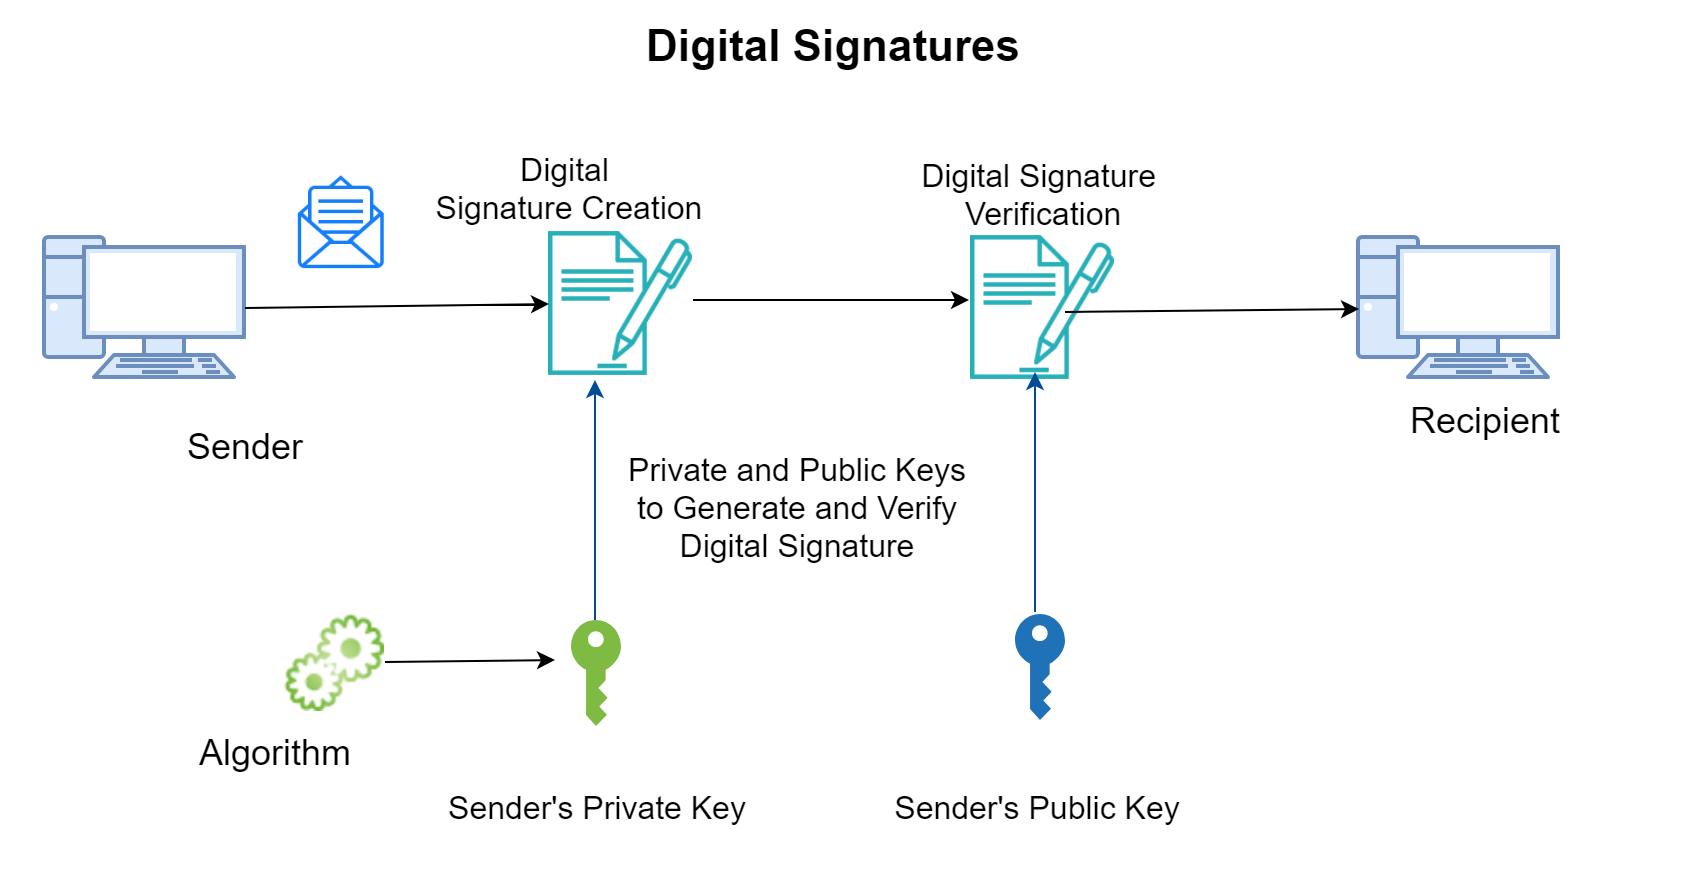
\includegraphics[width=1.0\textwidth]{Digital-Signature.png}
   \caption{Lược đồ chữ ký số \\ (Nguồn: https://yos.io/2018/11/16/ethereum-signatures/)}
\end{figure}

Trong các public blockchain như Bitcoin, Ethereum người ta dùng chữ ký số để định danh người gửi từ đó đảm bảo giao dịch không bị làm giả bởi một bên ác ý nào đó. ECDSA \cite{ECDSA} là thuật toán được sử dụng trong Bitcoin và Ethereum. Ngoài ra còn có EdDSA \cite{EdDSA} một thuật toán chữ ký số khác với rất nhiều ưu điểm.

\subsection{Merkle tree}

Merkle thực chất là một cây nhị phân, nơi mỗi nút lá là một giá trị hash của một block data, các nút không phải nút lá chứa giá trị hash của hai nút con. Giá trị hash ở nút gốc của cây được gọi là merkle root. 

\begin{figure}[H]
   \centering
   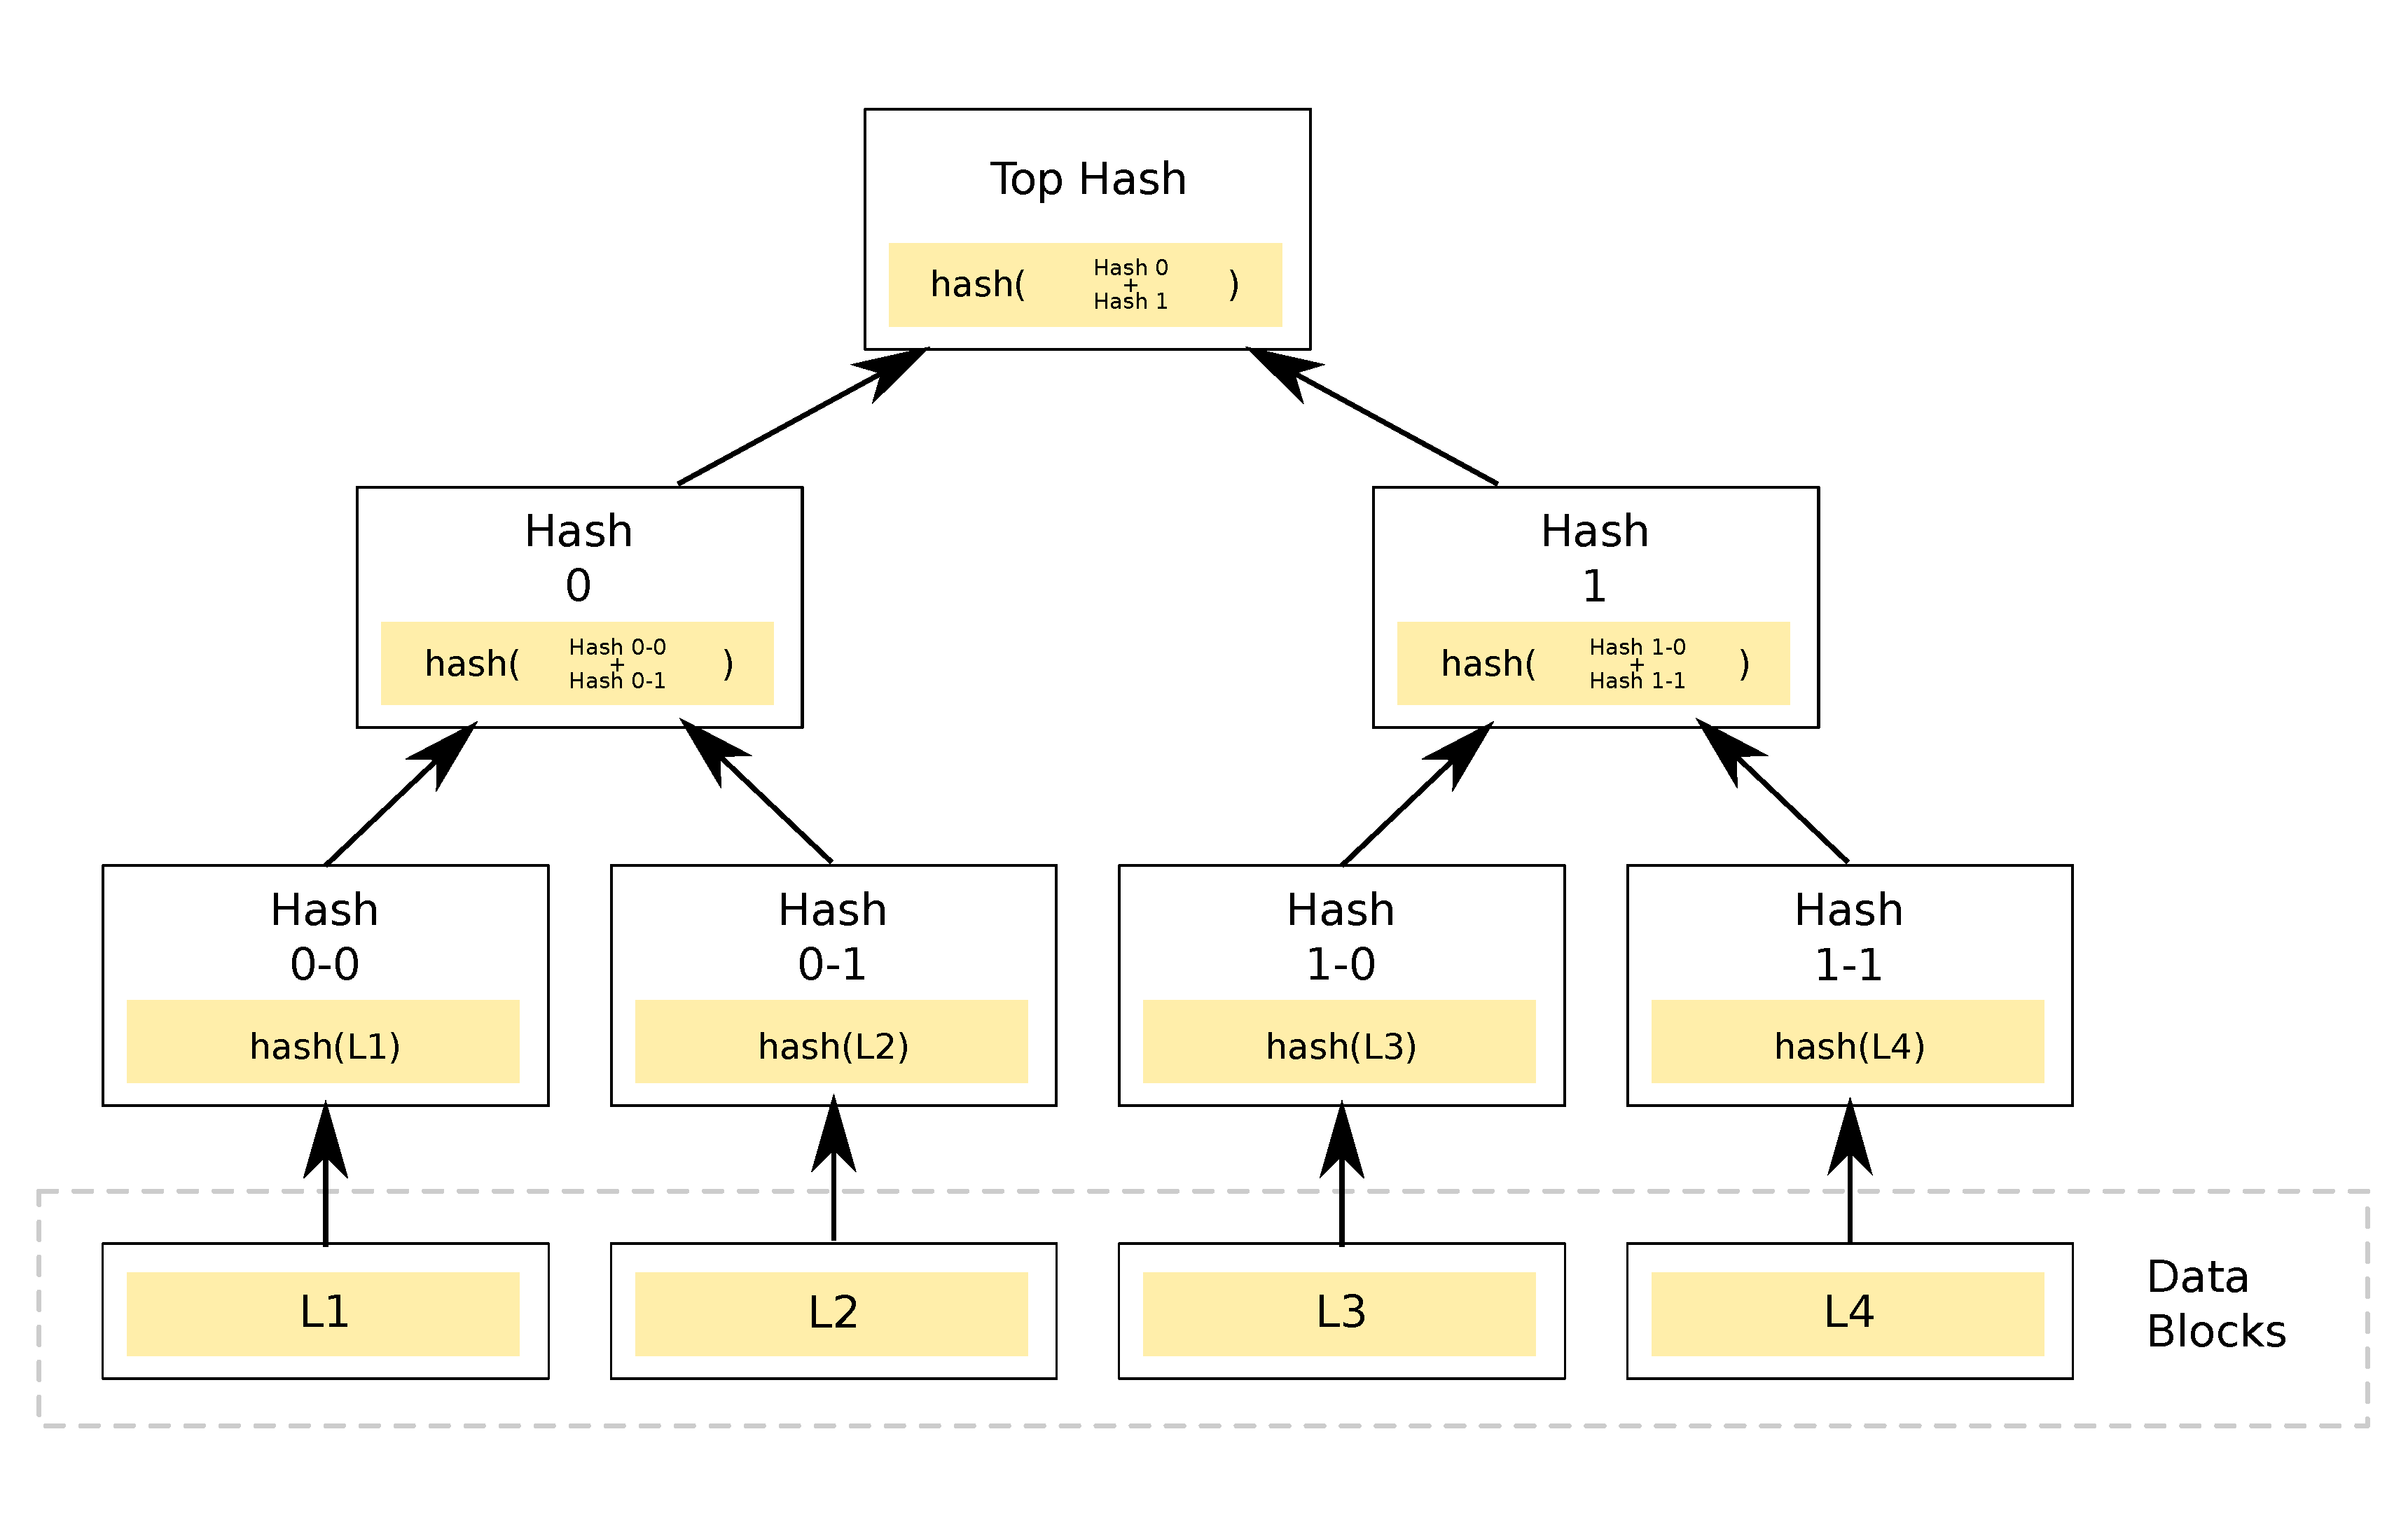
\includegraphics[width=0.9\textwidth]{Hash_Tree.pdf}
   \caption{Một ví dụ cụ thể về merkle tree (Nguồn: Azaghal)}
\end{figure}

Bằng việc lưu dữ liệu như trên, merkle tree cho phép người dùng có thể kiểm tra một block data có tồn tại trong tập hợp hoặc đúng thứ tự hay không rất hiệu quả. Bằng các xây dựng lại Merkle root bằng các tính toán lại các hash của các nút nằm trên đường đi từ nút lá chứa block data đó tới nút gốc.
\begin{figure}[H]
   \centering
   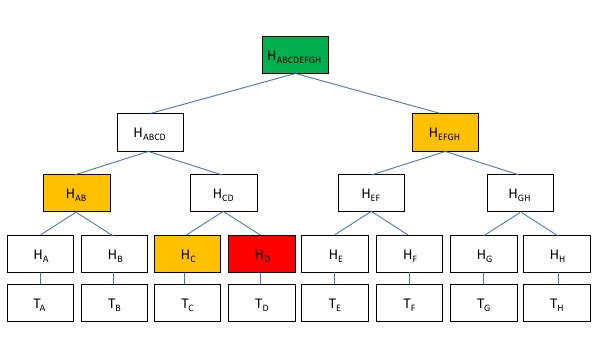
\includegraphics[width=0.9\textwidth]{merkle_tree_proof.jpeg}
   \caption{Verify data trên Merkle tree (Nguồn: Internet)}
\end{figure}

Ví dụ trong hình bên trên, ta có thể thấy trong hình bên trên, để verify $T_{D}$ có nằm trong cây hay không, ta sẽ tính toán lại Merkle root từ các giá trị $H_{C}$, $H_{AB}$, $H_{EFGH}$, nếu giá trị này chính là merkle root hiện tại thì ta chứng minh được $T_{D}$ thuộc Merkle tree. Trong trường hợp merkle tree là một cây nhị phân hoàn hảo, số lần chúng ta tính lại hash chỉ là $O(log_{2}(n))$. Tức số lượng data gửi kèm theo cho việc kiểm là rất nhỏ. 

\subsection{Zero Knowledge Proof}
Zero Knowledge Proof (ZKP) lần đầu được đề xuất năm 1985 bởi Shafi Goldwasser, Silvio Micali, and Charles Rackoff qua bài báo "The Knowledge Complexity of Interactive Proof-Systems", từ đó tạo nên một hướng nghiên cứu mới cho ngành khoa học bảo mật.

ZKP là một giao thức cho phép một bên tạm gọi là prover chứng minh với bên còn lại là verifier là họ biết một bộ giá trị $x$ thoả mảng một vấn đề nào đó nào đó mà không cần phải cung cấp bất cứ thông tin nào về giá trị $x$ cho verifier.

Một protocol ZKP phải thoả mảng 3 tính chất cơ bản sau:

\begin{itemize}
\item Completeness: nếu mệnh đề cần chứng mình là đúng, verifier chắn chắn được thuyết phục rằng nó đúng.
\item Soundness: nếu mệnh đề cần được chứng minh là sai, thì prover hầu như không thể thuyết phục được verifier là mệnh đề đó đúng, xác suất để trường hợp đó xảy ra là rất thấp.
\item Zero-knowledge: verifier hầu như không nhận được bất kỳ thông tin về lời giải từ prover.
\end{itemize}

\subsection{Zero-knowledge Succinct Non-Interactive ARgument of Knowledge}

\subsubsection{Định nghĩa và tính chất}
Zero-knowledge Succinct Non-Interactive ARgument of Knowledge(zk-SNARK) cũng là một giao thức Zero Knowledge Proof nhưng không cần sự tương tác giữa prover và verifier.

zk-SNARK thoả mãn các tính chất:
\begin{itemize}
\item Zero-knowledge: verifier không nhận bất cứ thông tin ngoài bài toán. 
\item Succinct: nghĩa là bằng chứng có kích thước nhỏ, dễ dàng kiểm chứng. 
\item Non-Interactive tức là không cần phụ thuộc vào các chu kỳ câu hỏi và cách kiểm chứng cho verifier là quy định trước trong giao thức. 
\item ARgument of Knowledge tức là gần như bạn gần không thể chứng minh cho verifier nếu bạn không kèm theo các kiến thức hổ trợ cho bằng chứng.
\end{itemize}

\subsubsection{Các bước thiết lập trong zk-SNARK}

Giả sử ta có bài toán chứng minh $F(\lambda) = x$. Ta thực hiện lần lược các bước sau để triển khai giao thức.
\begin{itemize}
\item Bước 1, Key Generator (G) nhận vào $\lambda$ sinh ra một bộ public key là proving key(pk) và verification key(vk). 
\begin{figure}[H]
   \centering
   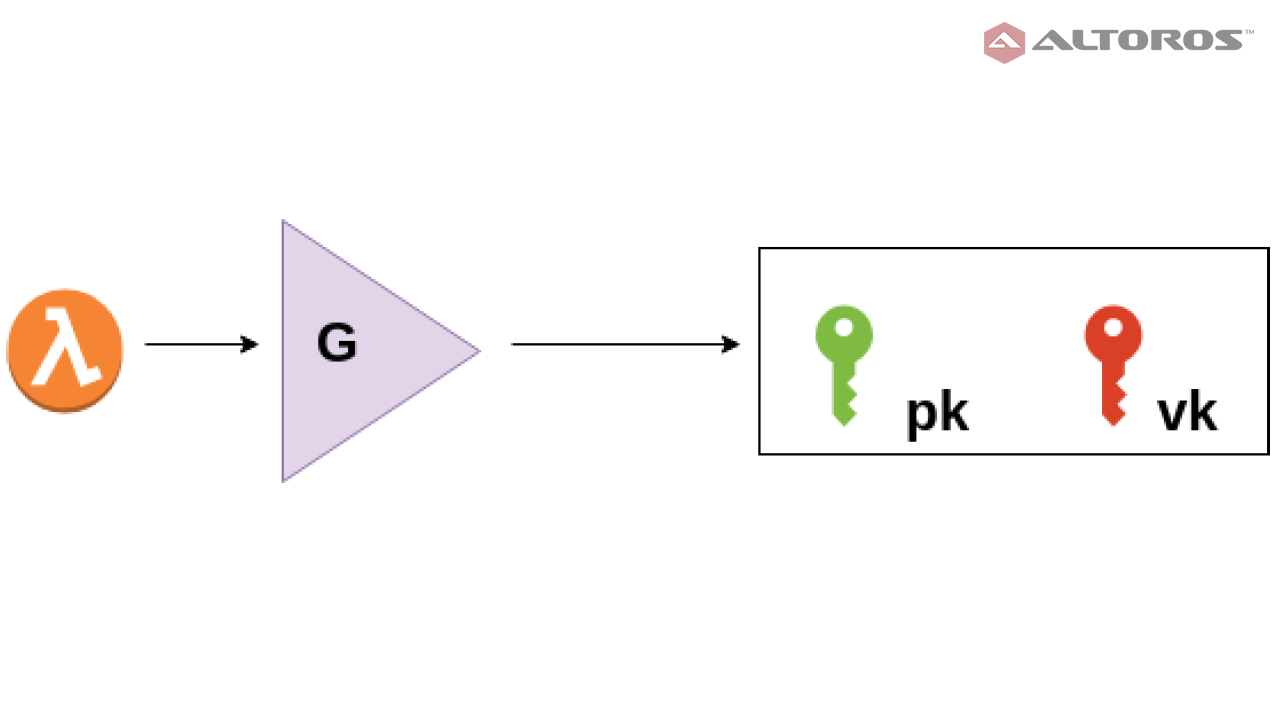
\includegraphics[width=0.7\textwidth]{blockchain-zkp-zk-snark-key-generator-v4.png}
   \caption{Gen key \cite{altoros}}
\end{figure}
\item Bước 2, Prover function(PF) lấy proving key(pk), public input x, và private input w và sinh ra một proof(bằng chứng). 
\begin{figure}[H]
   \centering
   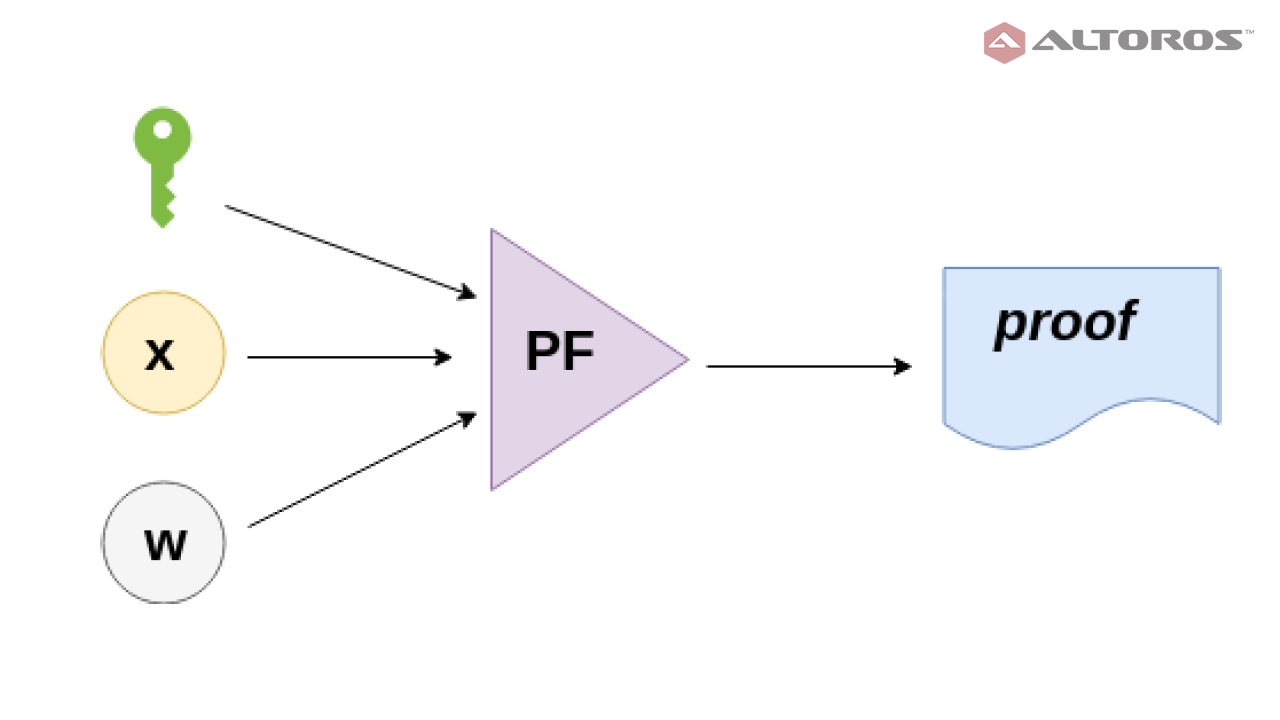
\includegraphics[width=0.7\textwidth]{blockchain-zkp-zk-snark-prover-function-v4.png}
   \caption{Gen proof \cite{altoros}}
\end{figure}
\item Bước 3, Verifier sẽ kiểm chứng proof có chính xác hay không bằng cách tính toán một hàm gọi là verifier function (VF) với input là vk, x và proof. Sau đó trả về kết quả Accept nếu đúng, Reject trong trường hợp ngược lại.
\end{itemize}
\begin{figure}[H]
   \centering
   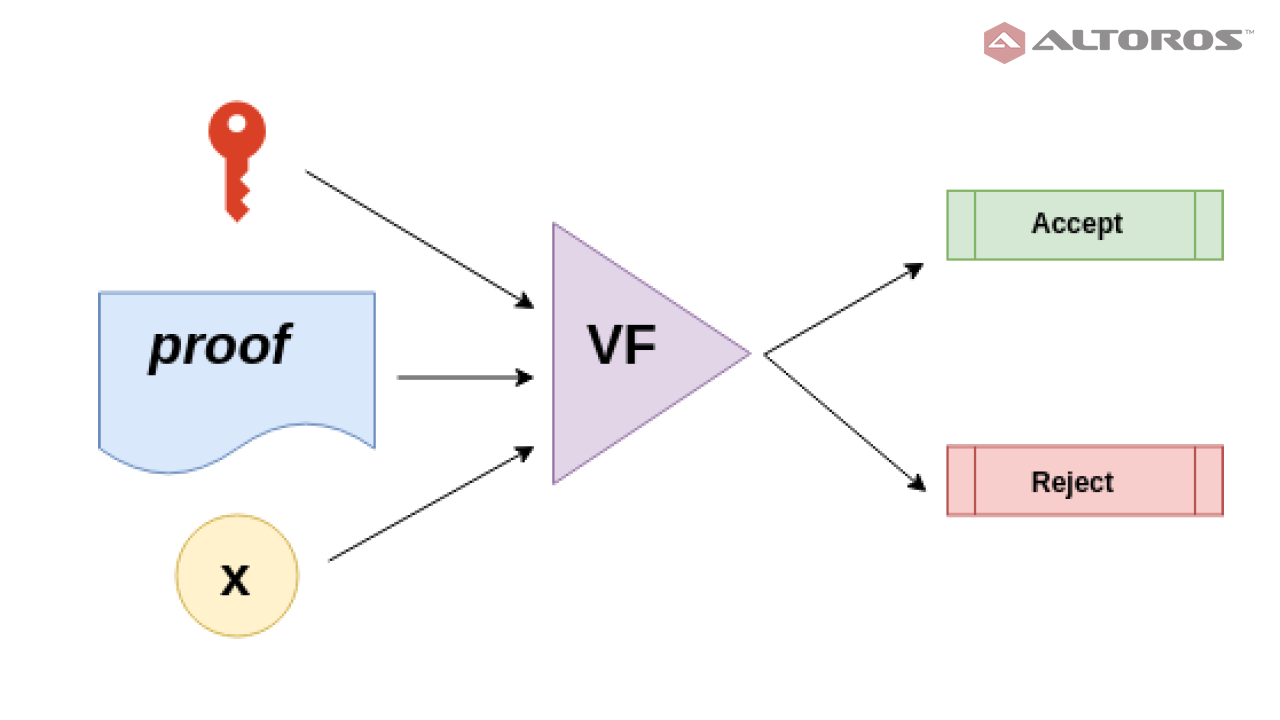
\includegraphics[width=0.7\textwidth]{blockchain-zkp-zk-snark-verifier-function-v4.png}
   \caption{Verify proof \cite{altoros}}
\end{figure}

Thật ra về mặt lý thuyết zk-SNARK phức tạp hơn như thế rất nhiều, nên tôi sẽ không trình bày tất cả chúng ở đây. Trong luận văn này tôi sử dụng giao thức Groth16 \cite{cryptoeprint:2016:260} được đề xuất bởi Jens Groth vào năm 2016. Mọi người có thể tham khảo thêm các thông tin về cơ sở toán học trong bài báo đó.

\section{Blockchain và các khái niệm cơ bản}
\subsection{Blockchain là gì}

Blockchain thường được định nghĩa như các khối (block) chứa thông tin được liên kết với nhau thông qua các hash, khối hiện tại chứa hash của khối trước. 

\begin{figure}[ht]
   \centering
   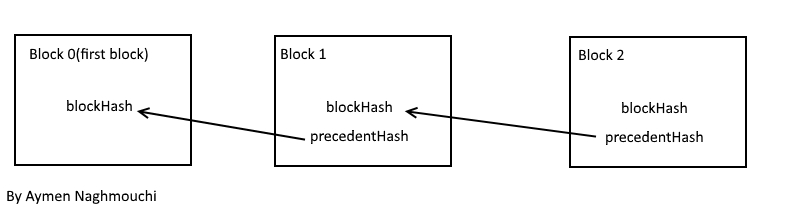
\includegraphics[width=0.7\textwidth]{blockchain-aymen.jpg}
   \caption{Một blockchain đơn giản}
   \source{https://github.com/aymen94/simple-Blockchain}
\end{figure}

Khi tạo ra hash cho block người ta hash các thông tin quan trọng bao gồm hash của khối trước đó. Nếu ta muốn sửa đổi thông tin trong một khối nào đó, ta phải đảm bảo liên kết khối được duy trì, điều này làm cho dữ liệu lưu trong blockchain khó bị sửa đổi. 

Đồng thời blockchain cũng là một cơ sở dữ liệu phân tán. Thay vì lưu trử dữ liệu trong một máy chủ cố định, blockchain sử dụng một mạng lưới P2P. Khi có một nút mới tham gia vào mạng, nó sẽ nhận đượ một bản sao dữ liệu của blockchain(ta gọi là sổ cái). Bản sao này tồn tại trên các nút tham gia blockchain network, nhưng nội dung của có là duy nhất trên một blockchain network. Tức là không tồn tại cùng lúc 2 sổ cái khác nhau trong cùng một thời điểm trong mạng blockchain. Để đảm bảo điều này blockchain cần một cơ chế đồng thuận.

\subsection{Cơ chế đồng thuận}
Trong blockchain, cơ chế đồng thuận là cơ chế được sử dụng để đảm bảo sự đồng thuận về một giá trị hoặc một trạng thái duy nhất của mạng. Trong trường hợp này nó đảm bảo mọi người tham gia blockchain network đồng ý với trạng thái của sổ cái, đảm bảo không có giao dịch bị làm giả.

Proof of Work có lẽ là cơ chế đồng thuận phổ biến nhất. Trong giao thức này các nút sẽ gộp các giao dịch thành một khối. Ta gộp các thông tin quan trọng trong khối lại và hash chúng lại với nhau, ta gọi đó là block hash. Bạn phải tìm được block hash thoả mảng một yêu cầu nào đó, ví dụ như 10 chữ số đầu của hash bằng đều bằng 0 chẳng hạn. Nhưng do dữ liệu trong khối là cố định, nên hàm hash luôn cho ra một block hash duy nhất. Do đó bạn phải cần có một giá trị biến thiên, ta sẽ tạo block hash bằng dữ liệu trong khối và giá trị biến thiên này. Bài toán lúc này là tìm giá trị biến thiên thoả mảng yêu cầu của mạng. Bài toán mà blockchain đặt ra cho node thường rất khó, đòi hỏi rất nhiều chi phí về tính toán để tìm ra lời giải. Quá trình thêm dữ liệu này có thể gọi là mint hay đào một khối mới. Hiện tại Ethereum cũng sự dụng cơ chế đồng thuận PoW.

\section{Ethereum Blockchain}
Trong phần này ta sẽ tổng quát về Etherum blockchain, đặc biệt là về cơ chế thanh toán cho việc thực thi giao dịch.
\subsection{Ethereum Blockchain là gì}
Ethereum blockchain là một nền tảng blockchain công khai, có khả năng tích hợp hợp đồng thông minh. Ether(ETH) là native cryptocurrency trong Ethereum. Người dùng sẽ dùng ETH để giao dịch với những người khác hoặc dùng để thanh toán cho những người đào khi người dùng muốn thực hiện một giao dịch.

\subsection{Ethereum Virtual Machine}
Ethereum Virtual Machine (EVM) là một máy ảo dùng chung trong Ethereum, nơi mà tất cả tất cả các người tham gia trên Ethereum lưu data và chấp nhận trạng thái đó. Các quy định về EVM được định nghĩa trong Ethereum yellow paper \cite{yellowpaper}.
\subsection{Account và Transaction}

Account(tài khoản) trong ethereum là một định danh với một ví chứa ETH. Account có thể gửi và nhận ETH thông qua giao dịch, đồng thời cũng có thể deploy hoặc tương tác với smart contract. Có 2 loại account là 

Transaction(giao dịch) đơn giản là một lệnh được ký bởi một tài khoảng nào đó. Giao dịch sẽ thay đổi trạng thái của Ethereum network.

Khi một transaction được gửi tới network, quy trình xử lý một transaction như sau: 

\begin{itemize}
  \item Dựa vào data của transaction, mà nó sẽ sinh ra một hash tương ứng.
  \item Transaction sẽ được gửi broadcast tới các node trong mạng và được đưa vào transaction pool với các transaction được gửi lên khác. 
  \item Người đào sẽ chọn các transaction và sắp sếp chúng tạo thành một block.Người đào sẻ chọn các transaction có gasPrice cao nhất vì đó là phí mà họ nhận được khi đào transaction.
  \item Transaction của bạn cũng sẽ nhận được một con số gọi là block confirmation định nghĩa cho số block trong blockchain được xử lý từ khi block chứa transaction của bạn được công nhận.
\end{itemize}

Lưu ý: chỉ việc thay đổi trạng thái của Ethereum mới tốn phí, việc đọc hay những thao tác không làm thay đổi trạng thái của Ethereum thì không tốn phí.

\subsection{Hợp đồng thông minh trong Ethereum}
Trong Ethereum, hợp đồng thông minh là các chương trình chạy trên Ethereum blockchain. Nó là tập hợp của các đoạn code (các hàm) hoặc dữ liệu (trạng thái) của một địa chỉ cụ thể nằm trên Ethereum blockchain. Người dùng hoặc các hợp đồng thông mình có thể tương tác với nhau thông qua các chức năng trong hợp đồng thông minh đó. Các đoạn code quy định chức năng này được định nghĩa khi hợp đồng được deploy lên Ethereum.

Hợp đồng thông minh trong ethereum có thể được phát triển qua các ngôn ngữ bật cao như Solidity \cite{solidity} hoặc Vyper \cite{vyper}. Khi biên dịch các trình biên dịch biên dịch các ngôn ngữ bậc cao này về đạng opcode, định dạng mà EVM có thể đọc và thực thi và lưu trên blockchain network. Khi có một tác nhân nào đó gọi tới hợp đồng thông minh, EVM sẽ chạy các opcode trong hợp đồng thông minh đó từ đó thay đổi trạng thái của Ethereum theo những gì trong hợp đồng quy định.

\subsection{Gas and gas price}
Gas tượng trưng cho một nổ lực tính toán bạn thực hiện dễ làm một công việc gì đó trên Ethereum. Ví dụ khi bạn tạo một transaction, transaction này làm một số công việc nhất định gì đó thì giá trị gas của transaction này tượng trưng cho lượng tài nguyên tính toán mà EVM sử dụng.

Như ta đã biết người dùng muốn thực hiện một transacion thì người dùng phải trả cho người đào một khoảng tiền nhất định. Số phí này được tính bằng công thức:

 \[fee = (gas\:cost) * (gas\:price)\]
 
Gas cost là lượng gas ta tiêu tốn cho transaction đó, còn gas price là số tiền được tính bằng wei(1 wei =$10^{-9}$ ETH) trả cho một gas trong transaction đó.

Trong Ethereum giá trị gas tối đa có thể thực hiện trong một block hiện này là vào khoảng 15 triệu gas(tính tới bản cập nhật Berlin).

\subsection{Tiêu chuẩn ERC-20 token}
ERC-20 \cite{ERC20} là một tiêu chuẩn cho Fungible Token (token có thể thay thế). Fungible Token có nghĩa là chúng có chung một thuộc tính làm cho các token này giống nhau. Ví dụ nếu bạn có 1 đô la thì nó có giá trị bằng 1 đô la, 5 đô la thì bằng 4 cộng 1 đô la, đó là các Fungible Token.

ERC-20 cung cấp một tiêu chuẩn cho việc tạo nhưng Fungible Token như vậy, cung cấp các giao diện chung cho tạo, giao dịch, truy vấn thông tin về các Fungible Token. Thay vì lưu trong account như ETH, ERC-20 token được lưu trong một smart contract. Tuỳ thuộc vào mục đích sử dụng mà ERC-20 token mang ý nghĩa khác nhau. ERC-20 token đơn giản và dễ sử dụng điều này làm cho nó rất phổ biến trong Ethereum. Điều đó kiến cho giao dịch ERC-20 trong Ethereum thường xuyên xảy ra.

\end{document}